% - How to build the CRT
\section{The Cosmic Ray Tagger panel}

This section covers technical aspects of the panels' components as well as manufacturing processes.

\subsection{The panel in a nutshell}
A panel consists of 16 scintillating bars embedded in an aluminium cover.
Each of the bars is prepared with two grooves, two \gls{wlsf}, a plastic endpiece and an electronics board with two embedded \gls{sipm}.
See figure \ref{fig:exploded_bar} for assembled and exploded assembly drawings of the scintillating bar.

\begin{figure}
  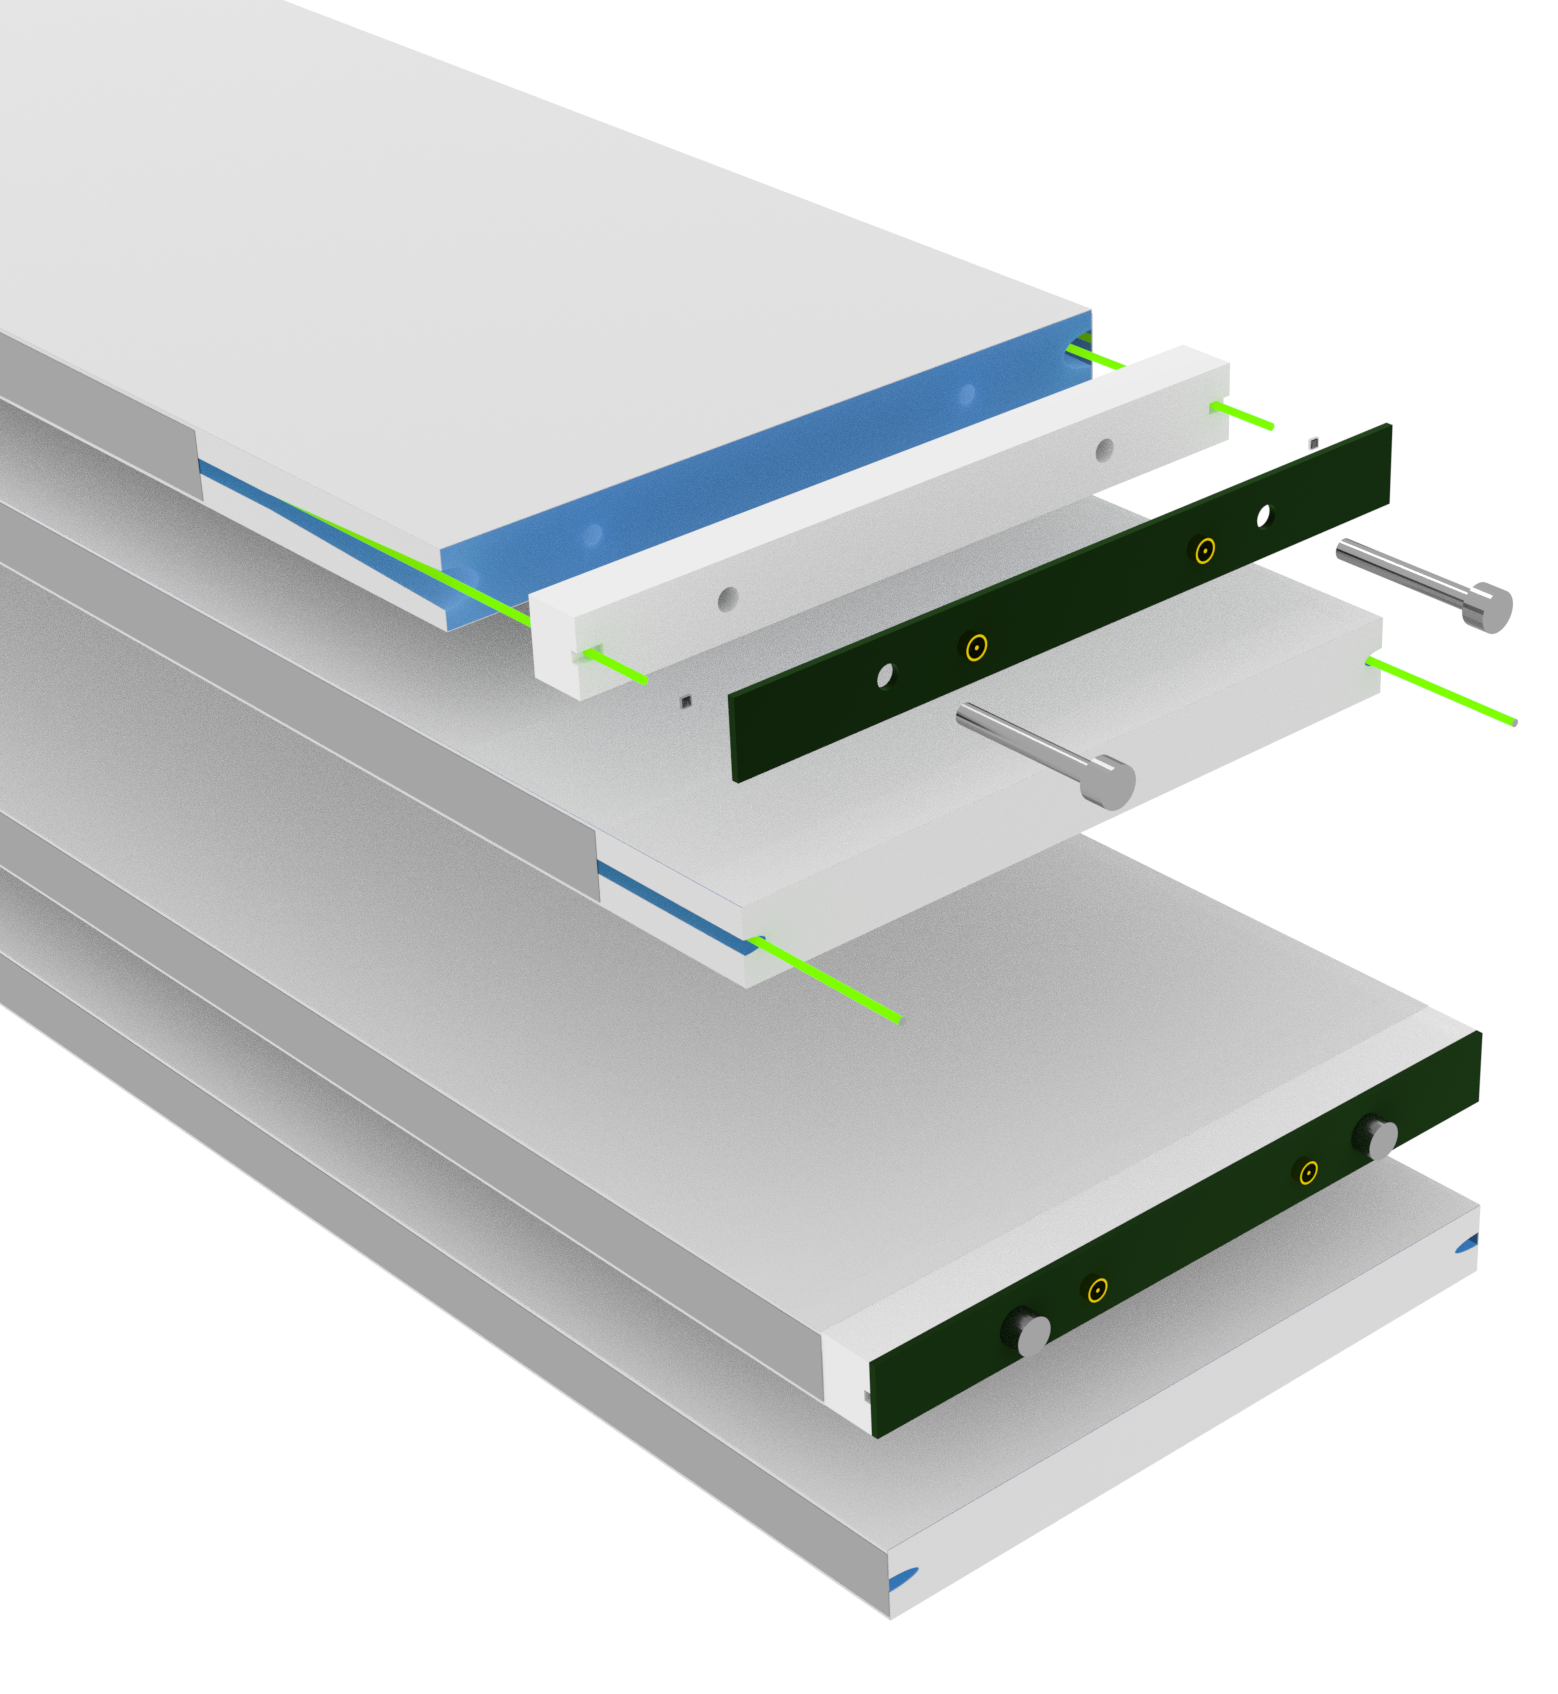
\includegraphics[width=\textwidth]{assembly}
  \caption{%
    Assembled and exploded views of front and rear ends of scintillating bars.
    The long sides of the bars (blue) are furnished with grooves containing the \glspl{wlsf} (fluorescent green) to guide the scintillation light to the \glspl{sipm} (black).
    The grooves are covered with mylar foil (gray).
    The plastic endpiece (white) serves as a physical guide and holder for the \glspl{wlsf}.
    The electronics and the enpiece are fixed to the bar with screws.
    Optical glue keep the \glspl{wlsf} and the mylar foil in place.
  }
  \label{fig:exploded_bar}
\end{figure}

When a high energy particle traverses the panel, it will most likely cross one of the scintillating bars\marginnote{This likelyhood depends on the fill factor of the panel} and induce the isotropical emission of photons.
These photons will be attenuated along their path in the material and reflected on the bars' walls until some of them reach the \gls{wlsf}.
The \gls{wlsf} are used for their light propagation properties and low attenuation coefficient, which allow some of the fluorescense photons to reach the \glspl{sipm}.
The photons arriving to the \gls{sipm} may induce the discharge of a cell in the \gls{sipm}, generating an observable signal.

\subsection{Aluminium shielding} The bars are covered with sheets of aluminium to shield the scintillating plastic and \glspl{sipm} from photons and charged particles.
The aluminium cannot dissipate all particle's energy, letting some photons and high energy particles through.
Knowing the kind of radiation tresspassing the detector is insightful, this is discussed for photons and charged particles.

\paragraph{Photons} are attenuated exponentially by the material along their path
\begin{equation*}
  I(x) = I_0 e^{-\mu x},
\end{equation*}
where $I_0$ is the intensity of the transmitted radiation at the interface and $x$ the perpendicular distance from the interface.

The attenuation depends on the energy of the photons, the nuclear structure and density of the material.
The attenuation coefficients for aluminium are displayed in figure \ref{fig:attenuation_coefficient_alu}.
\begin{figure*}
  \centering
  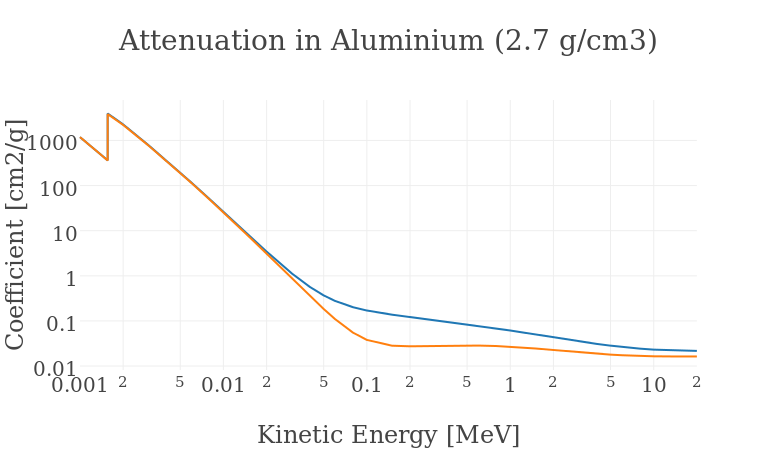
\includegraphics[width=.48\textwidth]{shielding/attenuation_photon}
  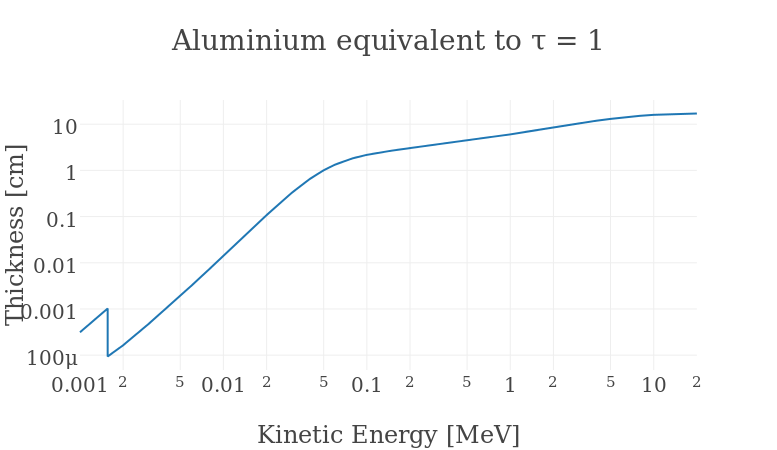
\includegraphics[width=.48\textwidth]{shielding/optical_depth}
  \caption{%
    The plot on the left displays the attenuation coefficient (blue) and energy absorption coefficient (orange) for photons in aluminium.
    The right plot displays the thickness of aluminium required to have an optical depth of one.
    Data used from NIST tables.
    Data source: \href{http://physics.nist.gov/PhysRefData/XrayMassCoef/tab3.html}{NIST Xray Mass Coefficients},
  }
  \label{fig:attenuation_coefficient_alu}
\end{figure*}

Since single photons can reach great depths in any material, it is more commonly used to express the thickness of a layer of material for incident radiation in optical depth
\begin{equation*}
  \tau = \mu x,
\end{equation*}
where $\mu$ is the attenuation coefficient and $x$ the thickness of the layer of material.

\marginnote{Assuming photons of the energy of 1.5MeV -- which is approximately the energy of the $\gamma$ photons resulting from \ce{^40K} undergoing electron capture in ambient radiation -- the mass attenuation coefficient of aluminium is $\mu_\rho = 0.05 \text{cm}^2 \text{g}^{-1}$ and therefore $\mu = \mu_\rho \rho = 0.135 \text{cm}^{-1}$.
The optical depth of $\tau = 1$ is reached with a $x = \frac{1}{\mu} = 7.4cm$ thick layer of aluminium.
For photons of energies above 0.1MeV, 2mm of aluminium is almost transparent.
}

\paragraph{Charged particles} For charged particles the penetration range can be estimated using a continuously slowing down approximation and the stopping powers of aluminium for every kind of particle
\begin{align*}
  R(E_0) &= \int_{E_0}^{0} \frac{1}{S(E)} dE \\
         &= \int_{E_0}^{0} -\frac{dx}{dE} dE.
\end{align*}

The high stopping power of aluminium for charged hadronic radiation stops heavy charged particles.
The nuclear contribution to energy loss for charged hadronic radiation is negligible.
Electrons lose almost all their kinetic energy to other electrons.
The radiation contributions of electrons start to be significant only for kinetic energies above 50MeV.
Using the stopping powers the ranges inside aluminium in depedence of their energy can be computed.
See figure \ref{fig:shielding} for an illustration of the stopping powers and ranges for electrons, protons and alpha particles in aluminium.

\begin{figure*}
  \centering
  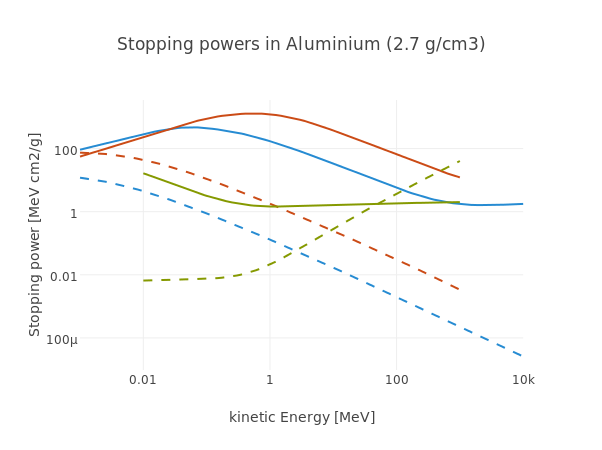
\includegraphics[width=.48\textwidth]{shielding/stopping_powers}
  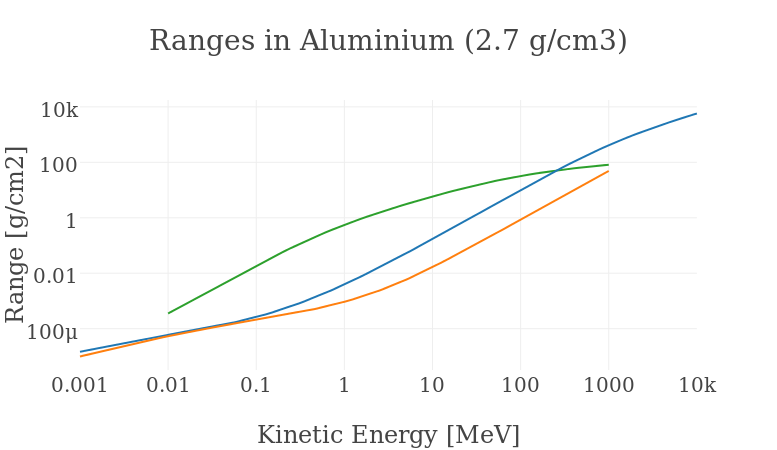
\includegraphics[width=.48\textwidth]{shielding/csda_ranges}
  \caption{%
    The stopping powers (left) and \gls{csda} ranges (right) are displayed for electrons (green), protons (blue) and alpha particles (orange).
    The radiative energy losses for electrons and nuclear contributions for the hadros are dashed.
    Data source: \href{http://physics.nist.gov/PhysRefData/Star/Text/ESTAR.html}{NIST ESTAR},
                 \href{http://physics.nist.gov/PhysRefData/Star/Text/PSTAR.html}{NIST PSTAR} \&
                 \href{http://physics.nist.gov/PhysRefData/Star/Text/ASTAR.html}{NIST ASTAR}
  }
  \label{fig:shielding}
\end{figure*}

\subsection{Scintillating bars}
The scintillating bars generate the grid of the \gls{crt} and yields light from the incident radiation.
A scintillator is a material which emmits light through luminescence when exposed to radiation.
When struck by ionizing radiation, a scintillator will absorb some of the radiation's energy and release the absorbed energy by light emission.\marginnote[2em]{Luc Beaulieu gave a good review on \href{https://vimeo.com/76977696}{Plastic Scintillation Detectors} at the AAPM 2013.}

The scintillation light originates from an organic fluor which is mixed into the plastic out of which the bars are produced.
The fluor excites into a metastable state, but its decay time is short\marginnote{The decay time is of the order of nano seconds.}, leading to almost no delay on the emission of the scintillation light.
The scintillation light is emitted isotropically from the radiation's incident point.
The components of the scintillating plastic are listed on table \ref{tab:material_safety_data_sheet}, the spectra of absorption and fluorescence of the scintillating components are displayed in figure \ref{fig:scintillator_graphs}.

\begin{table}
  \centering
  \begin{tabular}{ l l c }
    Ingredient                          & Synonym     & \% WT \\
    \hline
    Styrolution PS GPPS                 &             & 98.46 \\
    1,4-Diphenylbenzene                 & p-Terphenyl & 1.5   \\
    1,4-Bis(5-phenyl-2-oxazolyl)benzene & POPOP       & 0.04  \\
    \hline
    \\
  \end{tabular}
  \caption{%
    Composition / Information on ingredients of the scintillating plastic used for the bars of the \gls{crt}.
  }
  \label{tab:material_safety_data_sheet}
\end{table}

The bars come prepared with a thermal treatment, which increases the reflexion of light.
The size of the bars vary, depending on the dimensions of the module they are built in.
One side of the bars is faced to have a clean interface to fix the plastic endpiece to.
The grooves need to be cut open before glueing the \gls{wlsf} into them.

\begin{figure*}
  \centering
  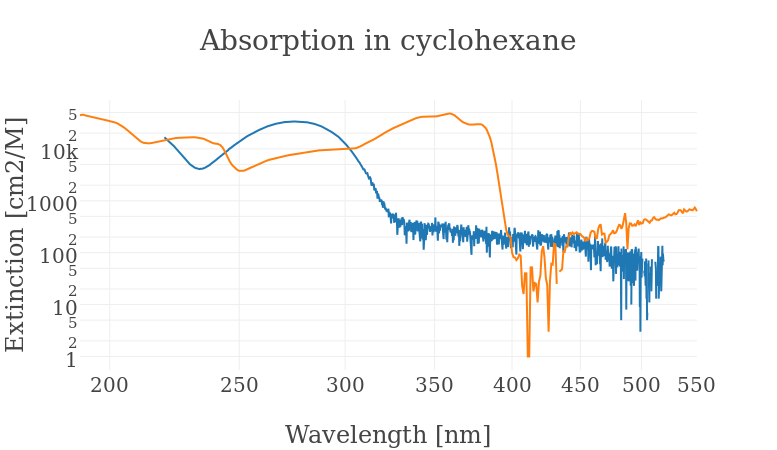
\includegraphics[width=.48\textwidth]{scintillators/absorptions_thin}
  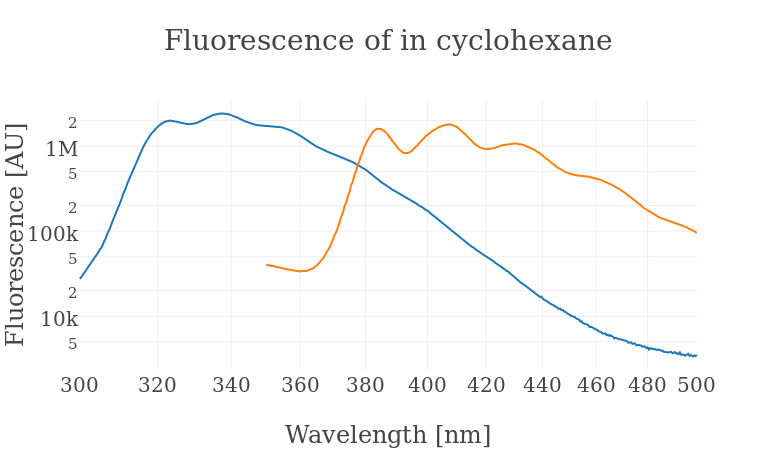
\includegraphics[width=.48\textwidth]{scintillators/fluorescences_thin}
  \caption{%
    (fttb)
    Optical absorption and fluorescence emission spectrum of p-Terphenyl (blue) and POPOP (orange) in cyclohexane.
    Data from PhotochemCAD package, version 2.1a (Du 1998, Dixon 2005), http://omlc.org/spectra/PhotochemCAD/
  }
  \label{fig:scintillator_graphs}
\end{figure*}

The scintillating bars are fixed to the aluminium sheets using double sided scotch tape.
The short sides of the panels are fixed to a prepared aluminium bar with screws.
The long sides of the panels are closed with U-shaped aluminium profiles, which are fixed with glue to the rest of the panel.
The gaps that might arise are closed with glue to minify the transision of photons.


\subsection{Wavelength shifting fibers}
Since light is collected through the fiber's cladding and a very low attenuation coefficient is needed, a \gls{wlsf} is used to guide the light from the scintillating bar to \glspl{sipm}.
\gls{wlsf} are very efficient light guides, since their emission and absorption spectrum is shifted, which leads to a very low attenuation coefficient.
The absorption and emission spectrum and the attenuation of the spectrum along a fiber are displayed on figure \ref{fig:wlsf_observations}.
Further technical details for the \gls{wlsf} Y-11 can be found on \href{http://kuraraypsf.jp/psf/ws.html}{kuraray's website} and its product catalogue.

\begin{figure*}
  \centering
  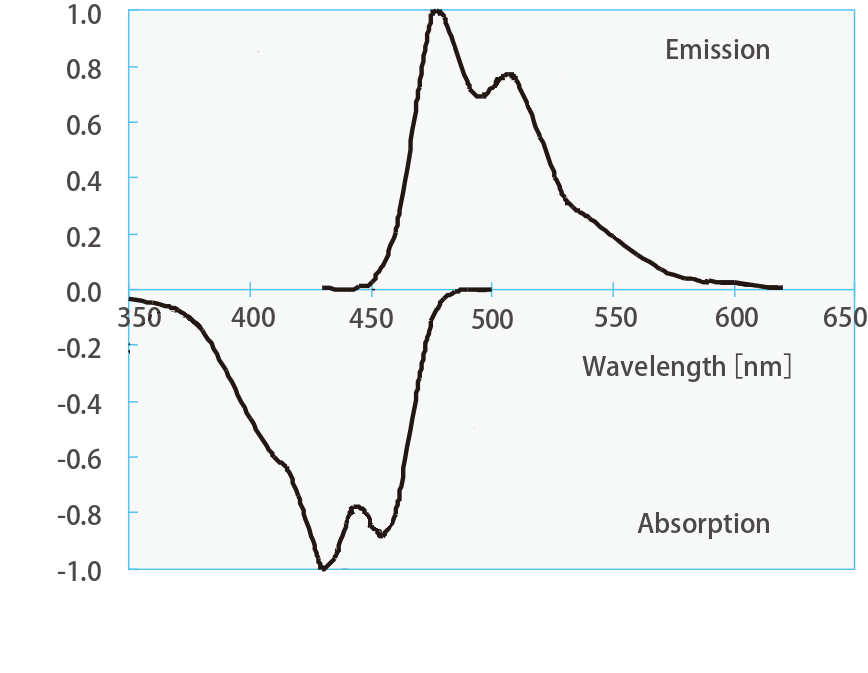
\includegraphics[width=.427\textwidth]{wlsf/absorption_emission_y11.png}
  \hspace*{1em}
  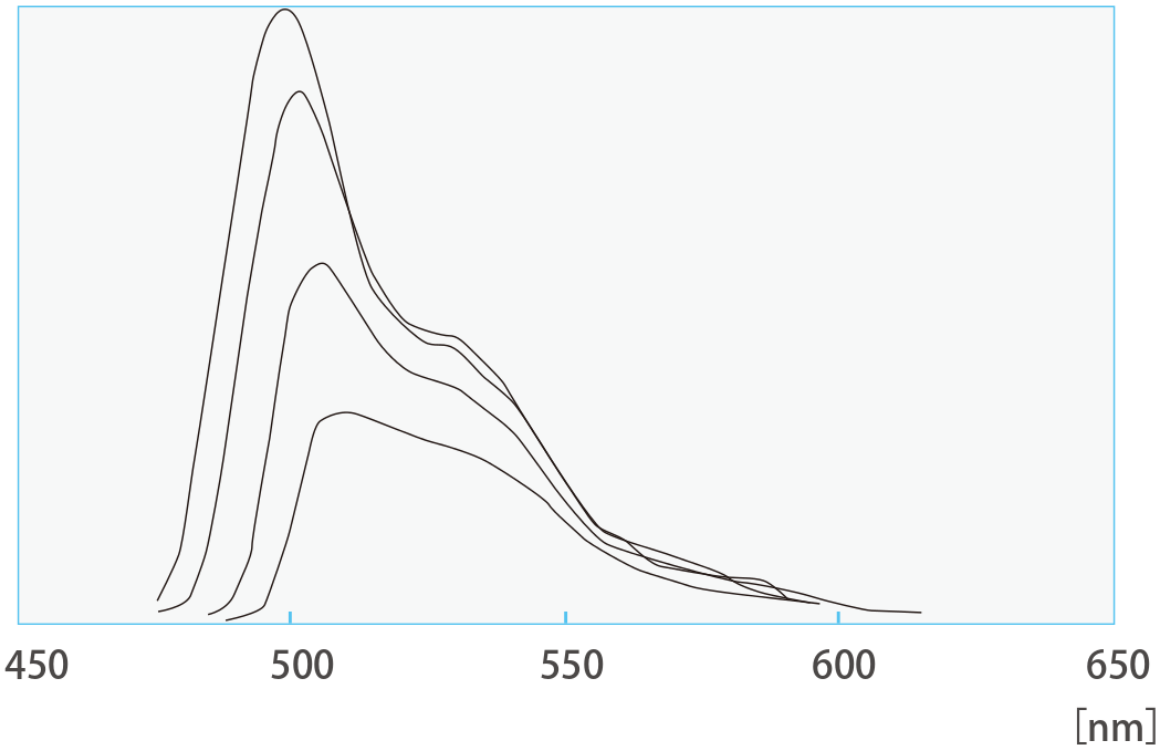
\includegraphics[width=.515\textwidth]{wlsf/attenuation_y11.png}
  \caption{%
    Absorption and emission spectrum of the \glspl{wlsf} displayed on the left shows peaking fluorescence emission at 476 nm and a maximal absorption at 430 nm.
    Attenuation of the spectrum of the \glspl{wlsf} on the right displays the spectrum at different distances (fttb 10, 30, 100, 300cm) from the source's incident point.
    The used light source to excite the fibers had a wave length of 430nm.
    Source: \href{http://kuraraysf.jp/pdf/all.pdf}{kuraray's product catalogue}
  }
  \label{fig:wlsf_observations}
\end{figure*}

The fibers are cut according to the length of the bars.
Both ends of the fibers are faced using a diamond-cutter to optimize the interface.
Aluminium is evaporated on the far end, to improve the reflexion of light.
The uncoated end is put on top of the \gls{sipm}, by using the plastic endpiece as physical guide and holder.
The fibers are glued to the groove using optical glue.

% Method
%\begin{figure*}
%  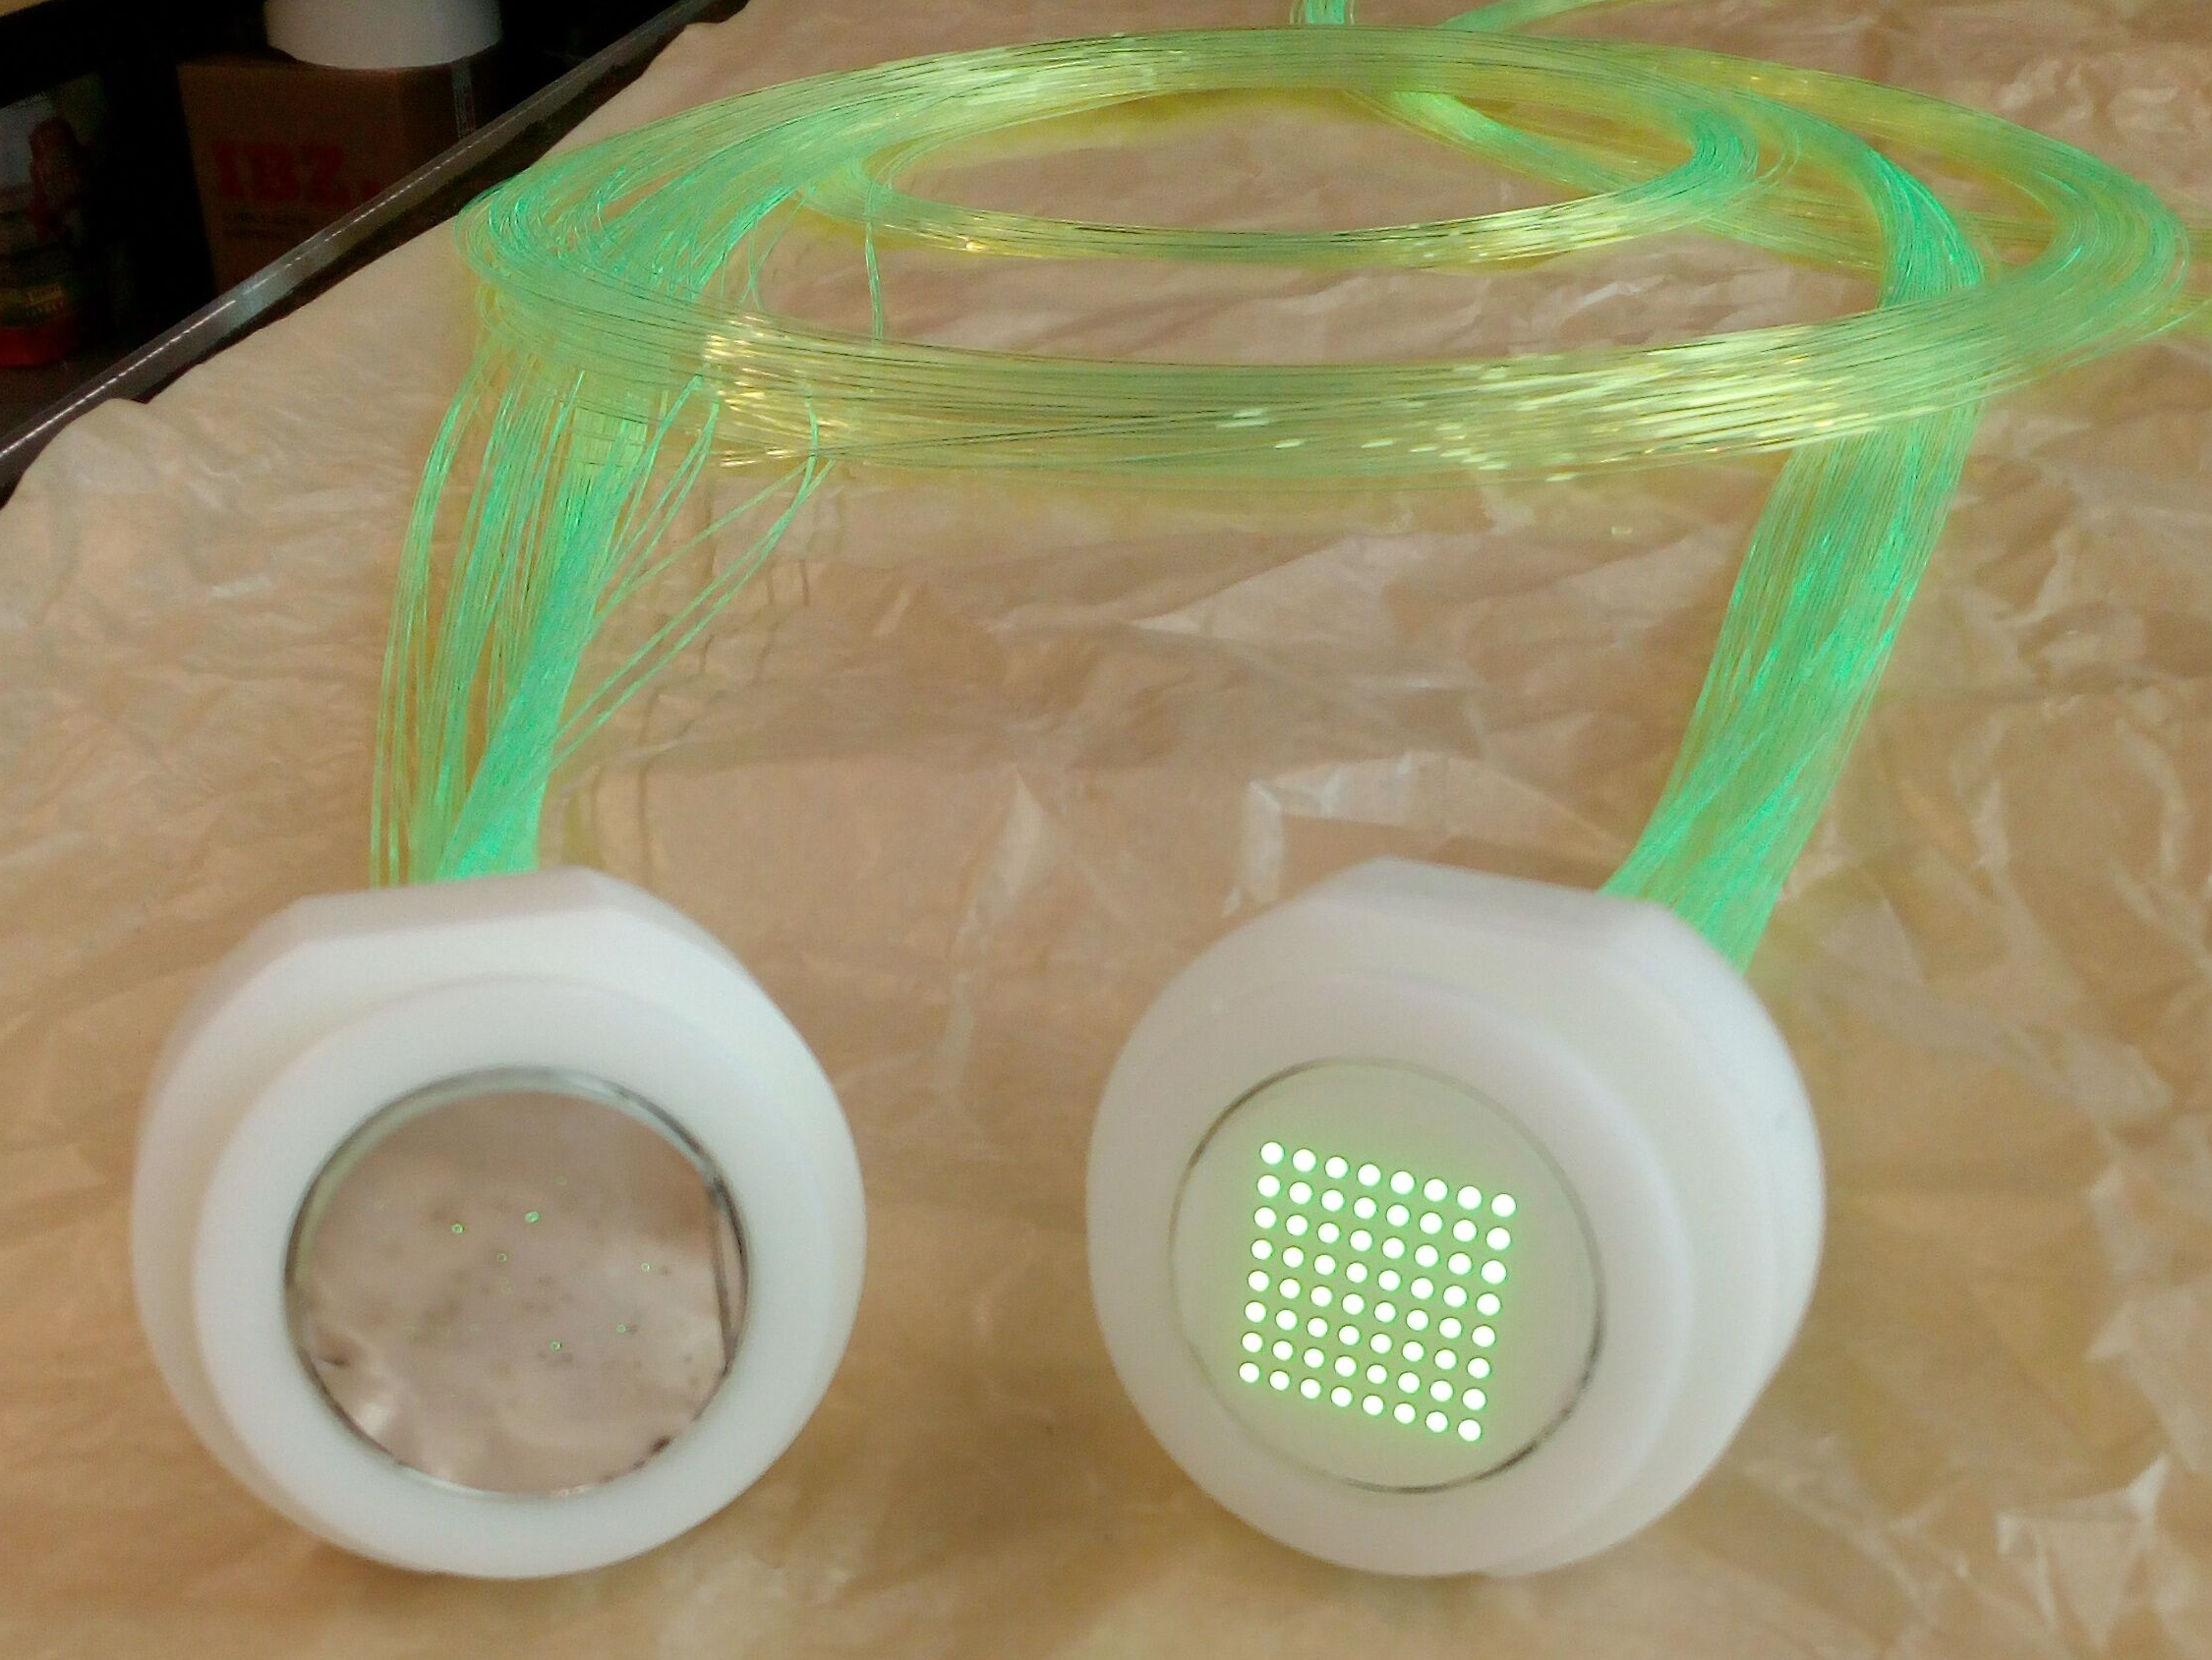
\includegraphics[width=\textwidth]{wlsf/fibers}
%  \caption{%
%    Fibers ready for assembly.
%    The fibers are fixed into plastic nests with optical glue, then both ends are diamond-cut.
%    One end is evaporated with aluminium to increase light reflexion.
%  }
%  \label{fig:exploded_bar}
%\end{figure*}
\clearpage
\subsection{Silicon photomultiplier}

A \gls{sipm} is an array of cells made of silicon, a well known semiconductor which is able to carry electrons and electron holes.
Each cell of the \gls{sipm} behaves like a diode, the electronic equivalent of a \gls{sipm} is displayed in figure \ref{fig:sipm_array_diodes}.

\begin{figure}
  \centering
  \begin{circuitikz}
    \node[ground] (g1) at (0, -1) {};
    \draw (0, -1) to[V=$V_\text{bias}$] (0, 1);

    \draw (0, 1) -- (1, 1);
    \draw (4, 1) to[D] (2.5, 1) to[R] (1, 1);
    \draw (4, 0) to[D] (2.5, 0) to[R] (1, 0) -- (1, 1);
    \draw (4, -1.5) to[D] (2.5, -1.5) to[R] (1, -1.5);
    \draw (1, 0) -- (1, -.5);
    \draw[densely dotted] (1, -.5) -- (1, -1);
    \draw (1,-1) -- (1,-1.5);

    \draw[densely dotted] (4, -.5) -- (4, -1);
    \draw (4, 1) -- (4, -.5);
    \draw (4, -1) -- (4,-1.5);
    \draw (4, 1) to[short,-o] (4.5, 1);
    \draw (4.5, 1) node[right] {$S_i$};

  \end{circuitikz}
  \caption{%
    Each branch of this electronic scheme represents a cell of the \gls{sipm}.
    All cells of the same crystal share the same bias voltage.
  }
  \label{fig:sipm_array_diodes}
\end{figure}

The charge carriers in the cells' silicon latice can be knocked out by incoming photons and drift to their appropiated electrodes if a field is applied.
With greater field the drift velocity increases, to the point where further charged carriers are knocked out.
With a sufficiently high voltage\marginnote{also called breakdown voltage} a photo electron leads to a self-sustaining avalanche.
A typical structure of a cell is shown in figure \ref{fig:sipm_structure}.

\begin{figure}
  \centering
  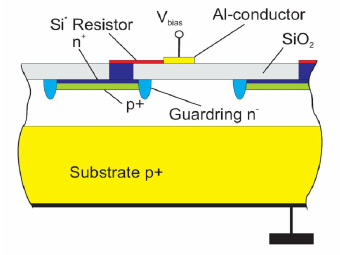
\includegraphics[width=.6\textwidth]{sipm_structure}
  \caption{%
    Typical structure of a \gls{sipm}'s cell.
    The cells are generally arranged on a 2 dimensional array.
    -- \copyright M. Teshima, \href{https://www.researchgate.net/publication/1764553_SiPM_Development_for_Astroparticle_Physics_Applications}{SiPM Development for Astroparticle Physics Applications}
  }
  \label{fig:sipm_structure}
\end{figure}

\Glspl{sipm} are run in Geiger mode, in which each cell behaves like a capacitance.
The amount of collected charge depends on the voltage applied to the \gls{sipm}'s cells.
Since the capacitances and the voltages are similar in within a \gls{sipm}, the collected charge is linearly proportional to the number of simultaneously discharged cells\marginnote{and therefore linearly proportional to the number of incoming photons!}.
The \glspl{sipm} used in the \gls{crt} are \glspl{mppc} produced by Hamamatsu.
More data can be found on table \ref{tab:sipm_specs}.

\begin{table}
  \centering
  \begin{tabular}{ l l r }
    \multicolumn{2}{l}{Parameter}                             & Value                 \\
    \hline
    \multicolumn{2}{l}{Effective photosensitive area}         & $1.3 \times 1.3 mm^2$ \\
    \multicolumn{2}{l}{Number of cells}                       & $667$                 \\
    \multicolumn{2}{l}{Geometrical fill factor}               & $62 \%$               \\
    \multicolumn{2}{l}{Breakdown voltage}                     & $65 V$                \\
    \multicolumn{2}{l}{Gain}                                  & $10^5 - 10^6$         \\
    \hline
  \end{tabular}
  \caption{
    Product specifications for Hamamatsu MPPC S12825-050.
    Source: Hamamatsu Product Flyer
  }
  \label{tab:sipm_specs}
\end{table}

